\documentclass{article}
\usepackage{graphicx} % Required for inserting images
\usepackage{amsmath}
\usepackage{esvect}
\usepackage{booktabs}
\usepackage{float}
\usepackage{enumerate}
\usepackage{hyperref}

\title{\textbf{Secure Multi-Party Computation
}Assignment 3 - Passive BeDOZa Implementation\textbf{}}
\author{Or Dinar \\
Liad Ackerman\\
\textbf{Late submission as approved by Dr. Akavia}}
\date{04.02.2024} \newline

\begin{document}

\maketitle

\section{Passive BeDOZa - Theory}

In this assignment we were given equation 3, and our task is to use the passive variant of BeDOZa protocol to securely compute the result. 
\newline
We chose to implement the protocol using boolean circuits.
Reminder:
\paragraph{Equation 3:}

$$
f_{\overrightarrow{a},4}(x_{1},x_{2})=\begin{cases}
			1 & \text{if $a_1x_1 + a_2x_2 \geq 4$ }\\
            0 & \text{otherwise}
		 \end{cases} \hspace{1cm} for \hspace{.25cm}  \overrightarrow{a} \in {\left\{ 0,1,2,3\right\}}^{2}
$$



\subsection{What does it do?}
The BeDOZA protocol uses the idea of \textit{Secret Sharing Schemes} in order to securely compute an operation of a logical gate. In boolean circuits, It does this by picking a random bit $r$ and computing $r \bigoplus x$ where $x$ is an input bit. \newline
In boolean circuits Secret Sharing Schemes have the following functions:
\begin{itemize}
  \item Shr($x$) - provided an $x$, pick a random bit (0 or 1) $r$ and return ($r$, $r \bigoplus x$).
  \item Rec($S_1,S_2$) - reconstructs the secret input buy applying $\bigoplus$ between the secret sharing themselves, then computing the XOR between the products.
  \item OpenTo(P,$S_1$) - returns $r\bigoplus r \bigoplus x$ to the party P, which, in turn, is the secret $x$.
  \item Open($S_1$) - returns $r\bigoplus r \bigoplus x$ to all parties.
\end{itemize}
\newpage


\subsection{Implementation}
In our implementation of the boolean circuit for Equation 3, we defined a function for each logical gate, as well as functions for the \textit{Secret Sharing Scheme}'s operations. The functions in the python implementation are the following:

\begin{itemize}
  \item shr(secret)
  \item recSelf(secret)
  \item rec(x, y)
  \item openTo(secret)
  \item XOR(x, y)
  \item XORconst(x, c)
  \item AND(x, y)
  \item ANDconst(x, c)
  \item OR(x, y)
  \item twoBitMulti(num1,num2)
  \item fourBitAdder(num1,num2)
  \item boolianCircuit(a1,a2,x1,x2)
\end{itemize}
\newpage
\subsection{Equation 3's Boolean Circuit}
We'll provide an image of the boolean circuit for Equation 3 for reference.
\begin{figure}[H]
    \centering
    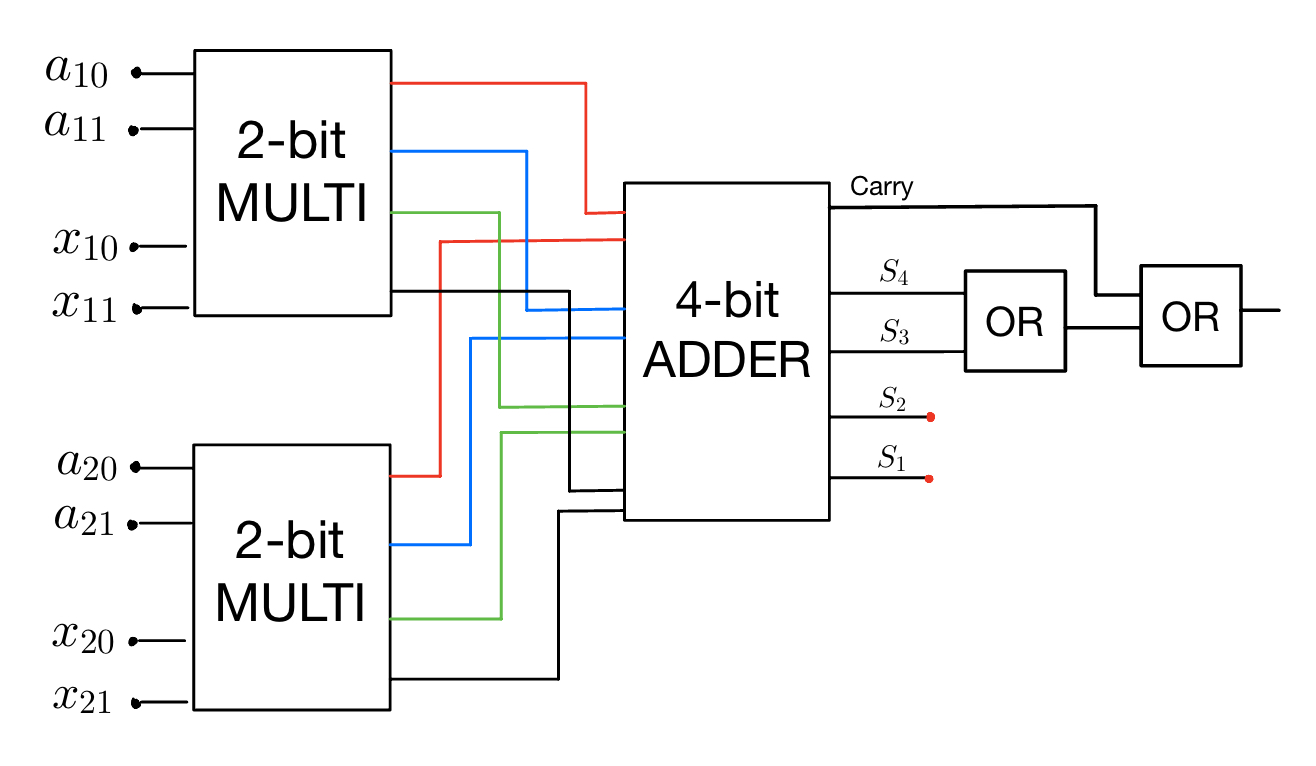
\includegraphics[width=1\linewidth]{FinalBooleanCircuit.jpeg}
    \caption{Boolean circuit that represents $Equation$ $3$.}
    \label{fig:enter-label}
\end{figure}

We also recall that the implementation of 2-bit Multiplier and 4-bit Adder were as following:
\begin{figure}[H]
    \centering
    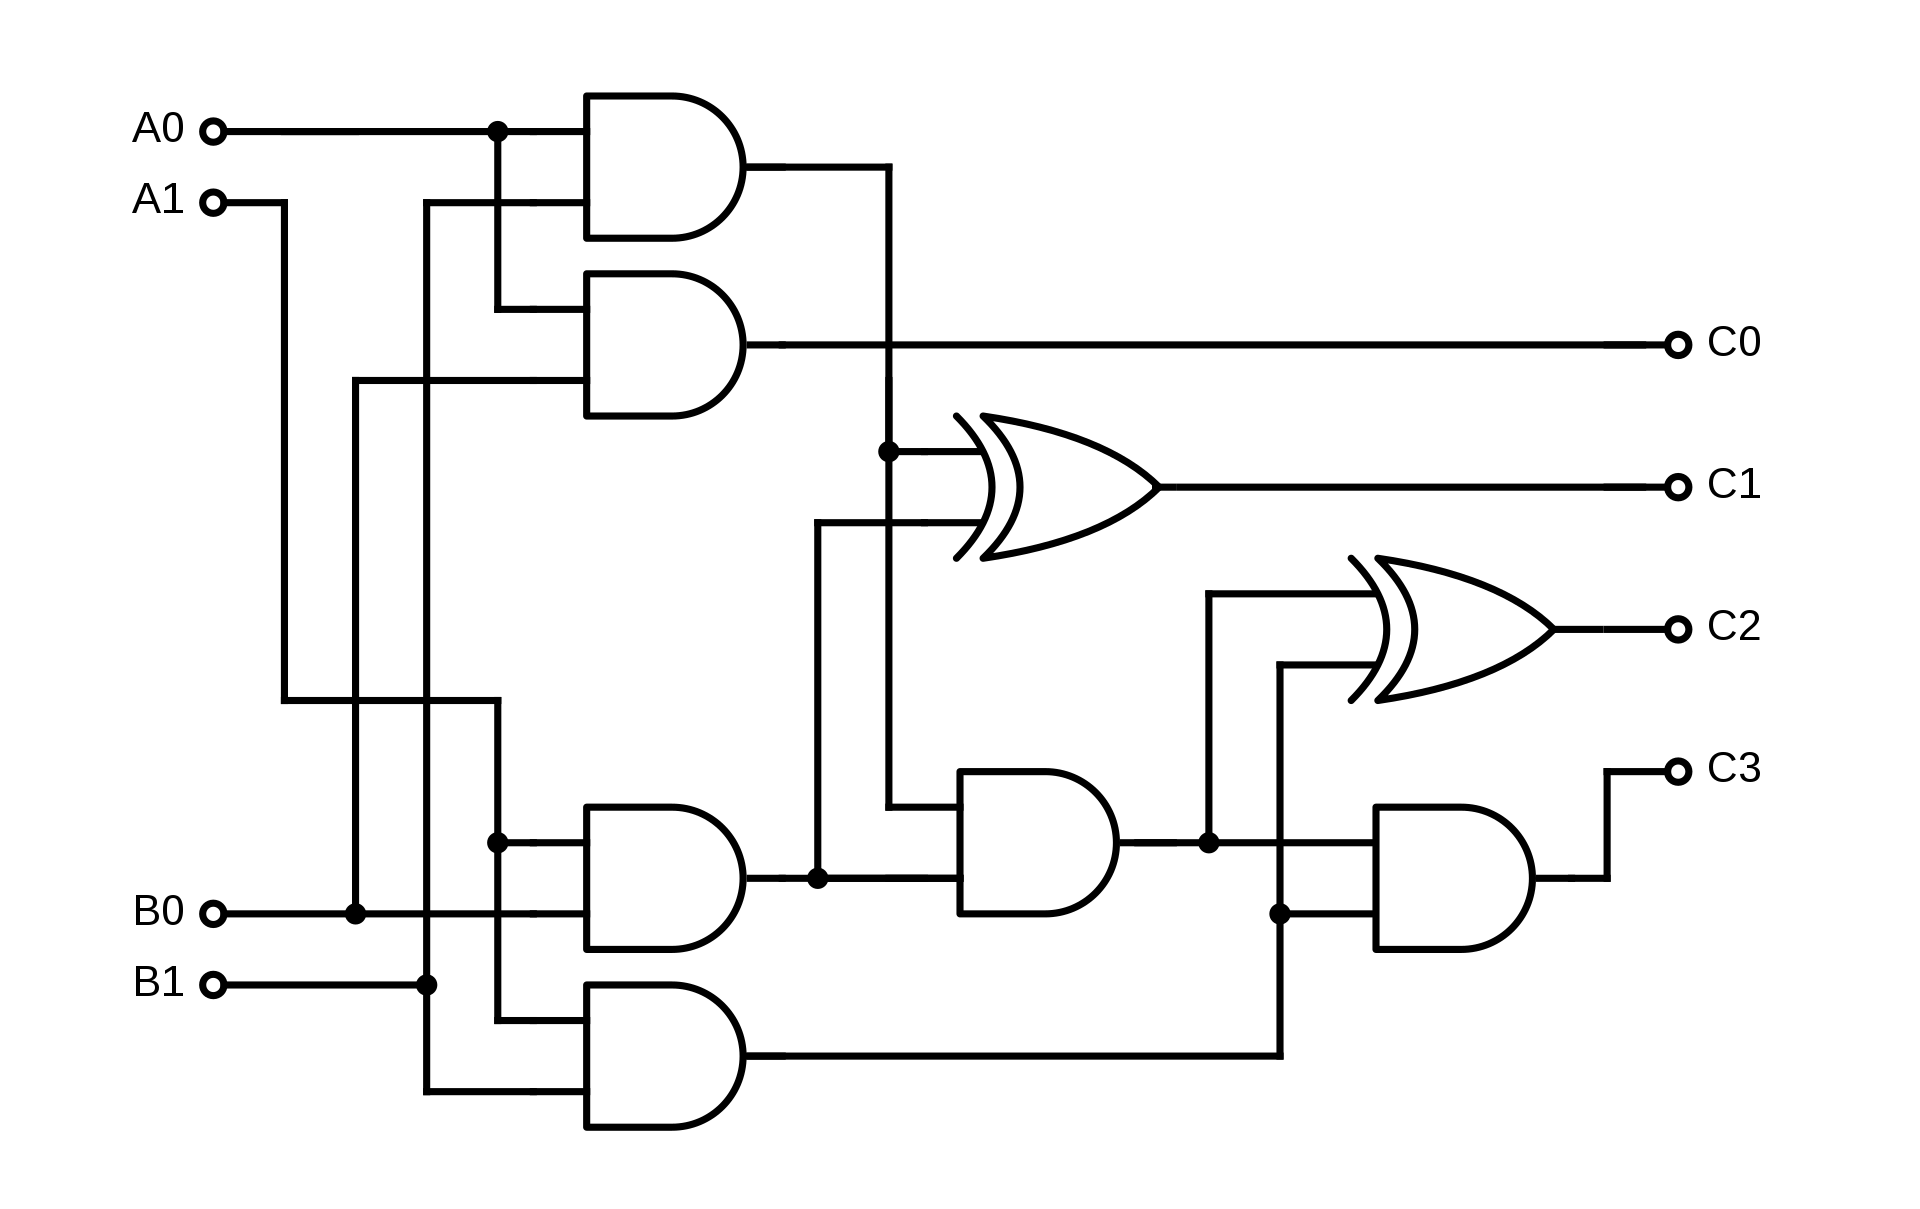
\includegraphics[width=0.75\linewidth]{1920px-Binary_multiplier.svg (1).png}
    \caption{2-bit Multiplier.}
    \label{fig:enter-label}
\end{figure}

\begin{figure}[H]
    \centering
    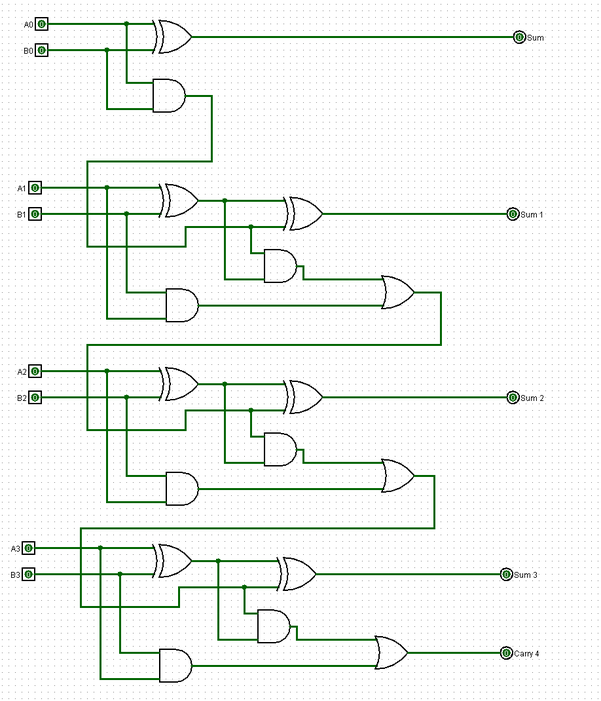
\includegraphics[width=1\linewidth]{F3D2GZ2KNVR5S0C.png}
    \caption{4-bit Adder.}
    \label{fig:enter-label}
\end{figure}
\newpage
furthermore, since only AND and XOR gates are allowed, we also implemented the OR gate using AND and XOR gates, as shown in Figure 4 below:

\begin{figure}[H]
    \centering
    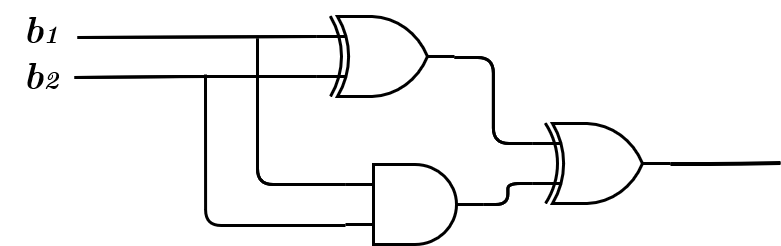
\includegraphics[width=1\linewidth]{OR GATE.png}
    \caption{OR gate using XOR and AND gates}
    \label{fig:enter-label}
\end{figure}

In the attached python file, we implemented each of the calculations above as functions, such that 2-bit Multiplier receives two 2-bit numbers - each of those bits is masked by \textit{secret sharing}, and returns a secret shared 4-bit product {$a_ix_i$.} While 4-bit Adder receives two \textit{secret shared} products from 2-bit Multiplier, and returns secret shared 5-bit sum $[Carry,bit4,bit3,bit2,bit1]$. We also recall that the sum is greater or equal to 4 (given threshold) if either one of $[Carry, bit4,bit3]$ is 1, hence the last two OR gates at the end. 


All in all, we constructed a Boolean circuit for the function in Equation 3. It receives 4 Secret Shared bits for $a$ and 4 Secret Shared bits for $x$ and computes the equation.
\end{document}
